%
% Tesi D.S.I. - modello preso da
% Stanford University PhD thesis style -- modifications to the report style
%
%%%%%%%%%%%%%%%%%%%%%%%%%%%%%%%%%%%%%%%%%%%%%%%%%%%%%%%%%%%%%%%%%%%%%%%%%%%
%                                                                         %
%			TESI DOTTORATO                                                %
%			______________                                                %
%                                                                         %
%			AUTORE: Andrei Ciulpan                                        %
%                                                                         %
%			Ultima revisione: 4.05.2019                                  %
%                                                                         %
%%%%%%%%%%%%%%%%%%%%%%%%%%%%%%%%%%%%%%%%%%%%%%%%%%%%%%%%%%%%%%%%%%%%%%%%%%%
%
%
\documentclass[12pt]{report}
%    \renewcommand{\baselinestretch}{1.6}      % interline spacing
%
% \includeonly{}
%
%			PREAMBOLO
%
\usepackage[a4paper]{geometry}
\usepackage{amssymb,amsmath,amsthm}
\usepackage{graphicx}
\usepackage[hyphens,spaces,obeyspaces]{url}
\usepackage{hyperref}
\usepackage{epsfig}
\usepackage[italian]{babel}
\usepackage{tesi}
\usepackage{afterpage}

\addto{\captionsitalian}{%
	\renewcommand{\bibname}{Sitografia}
}

\newcommand\blankpage{%
	\null
	\thispagestyle{empty}%
	\addtocounter{page}{-1}%
	\newpage}

% per le accentate
\usepackage[utf8]{inputenc}
%
\newtheorem{myteor}{Teorema}[section]
%
\newenvironment{teor}{\begin{myteor}\sl}{\end{myteor}}
%
%
%			TITOLO
%
\begin{document}
\title{Sistema Accessi IoT}
\author{Andrei CIULPAN}
\dept{Corso di Laurea in Informatica} 
\anno{2018/2019}
\matricola{872394}
\relatore{Dott. Andrea TRENTINI}
\correlatore{Marco LANZA}
\afterpage{\blankpage}
% 
%			DEDICA
%
\beforepreface

{\hfill \footnotesize {\sl Ringrazio i miei genitori e la nonna per il sostegno e per la pazienza che hanno avuto.}}
\vskip 0.8cm
{\hfill \footnotesize {\sl Ringrazio i miei amici e compagni di università per aver reso l'esperienza più bella e soprattutto più facile.}}
\vskip 0.8cm
{\hfill \footnotesize {\sl Ringrazio i miei tutor e colleghi per avermi dato la possibilità di crescere e concludere la mia esperienza universitaria.}}
\vskip 0.8cm
{\hfill \footnotesize {\sl Un ringraziamento speciale a Elena per essere riuscita a farmi sorridere e a tirarmi su il morale in ogni giorno con la sua presenza nella mia vita.  Un altro ringraziamento a lei per la revisione della tesi.}}
       

\afterpreface

% 
%			CAPITOLO 1: Intro
\chapter{Introduzione}
\label{cap1}
%

Il controllo accessi è un sistema di protezione che permette l'accesso solo a determinate persone per via di qualche procedura di autenticazione: nel mondo fisico si può parlare di una semplice serratura (storicamente il sistema piu' utilizzato in assoluto) che può essere aperta solo dalle persone in possesso della chiave, mentre nel mondo dell'informatica si può notare l'enorme utilizzo delle procedure di autenticazione (login) che aiutano il sistema, tramite l'inserimento di un nome utente e password, a determinare automaticamente se una persona è autorizzata ad accedere alle risorse del sistema stesso.

Il controllo accessi\cite{controllo_accessi} è un tema molto sviluppato nel campo della sicurezza sia fisica che informatica: è stato segnalato che nel 2017, per il secondo anno consecutivo, il mercato del controllo accessi ha avuto la crescita piu' rapida nell'industria della sicurezza fisica\cite{crescita_controllo_accessi}. E' anche un sistema onnipresente, utilizzato in ospedali, fabbriche, supermercati, aziende, sistemi di trasporto pubblico (e.g l'ATM di Milano), case e tanti altri campi.  

La tesi si propone di trattare un sistema ibrido in cui il mondo fisico e il mondo informatico lavorano insieme: attraverso sensori ed attuatori è possibile avere la comunicazione tra i due mondi. 
Si tratta di un sistema IoT (Internet of Things), ovvero un sistema in cui la connessione Internet viene estesa anche al mondo degli oggetti fisici (smart objects\cite{smart_objects}) di uso comune. Gli oggetti si rendono riconoscibili e acquisiscono intelligenza grazie al fatto di possedere una o piu' delle seguenti funzionalità: identificazione, localizzazione, diagnosi di stato, interazione con l'ambiente circostante, elaborazione dati e ovviamente connessione.
Gli oggetti intelligenti di un sistema IoT sono normalmente dotati di un processore embedded, sensori e attuatori e sono in grado di agire sui dati raccolti dall'ambiente e, ancora piu' importante, mandare questi dati in rete dove possono poi essere analizzati\cite{IoT}. Un semplice esempio di un sistema IoT si può trovare in Figura 1.

Le seguente sezione di questo capitolo introdurrà il progetto stesso (denominato SimSim) che poi verrà dettagliato nei prossimi capitoli.

\begin{figure}
	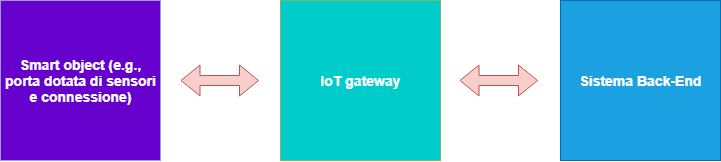
\includegraphics[width=\linewidth]{./img/iot_diagram.png}
	\caption{Esempio di sistema IoT}
	\label{fig:iot1}
\end{figure}

%
\section{Panoramica del progetto}
%
L'attività principale del tirocinio è la realizzazione di un sistema di controllo accessi basato su Arduino, 
da applicare presso varchi. Il sistema è in grado di funzionare con diverse modalità di riconoscimento quali RFID, controllo remoto e tastierino numerico. A seguito di ogni accesso avvenuto con successo, il sistema salva il log in un database remoto (in LAN) via WiFi. 

Parallelamente il sistema possiede un'interfaccia per l'utente utilizzatore (in questo caso un sito web) dove può accedere ai log degli accessi, oltre a un database per poter gestire i soci e le tessere RFID dell'azienda. Il server web è sviluppato utilizzando NodeJS e MongoDB (per il database) ed è hostato su un Raspberry Pi 3B+.

Nelle figure 2 e 3 si possono trovare rispettivamente un diagramma dei casi d'uso e un diagramma di flusso del sistema.


\begin{figure}
	\center{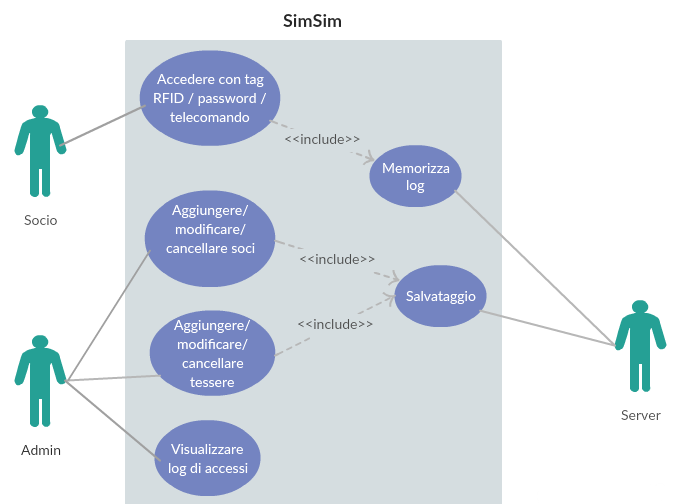
\includegraphics[width=0.6\linewidth]{./img/usecase.png}}
	\caption{Casi d'uso del sistema}
	\label{fig:usecase}
\end{figure}

\begin{figure}
	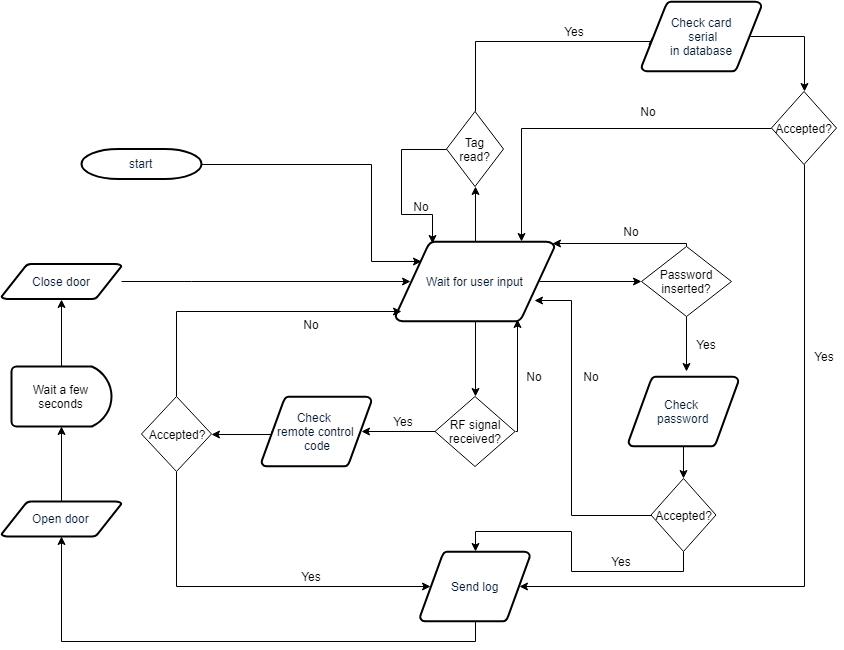
\includegraphics[width=0.9\linewidth]{./img/flowchart.png}
	\caption{Diagramma di flusso del sistema}
	\label{fig:flux}
\end{figure}


%			CAPITOLO 2: Hardware
\chapter{Hardware}
\label{cap2}
%
Schema circuitale completo?
%
\\
\section{Raspberry Pi}
%
\section{Arduino UNO}
%
\section{RTC (perchè la Raspberry Pi non ce l'ha ed è privo di connessione Internet)}
%
\section{Ricevitore RF}
Un po' di matematica sulle antenne
%
\section{Servomotore}
PWM
\\ 
\section{RFID}
%
\section{Display LCD 16x2}
%
\section{Keypad}
%
\section{ESP-01}
%
Problematiche
\\
Alternative
\section{Protocolli di trasmissione dati}
\subsection{Logica IoT}
%
\subsection{Comunicazione Wi-Fi in rete locale. Parlo anche del protocollo HTTP?}
%
\subsection{I2C}
%
\subsection{SPI}
% 
%			CAPITOLO 3: Software
\chapter{Software}
\label{cap3}
%
%
%
\section{Strumenti dello sviluppatore}
Arduino IDE
\\
Node.js
\\
Postman
\\
MongoDB 
\\
Per i linguaggi di programmazione metto solo un riferimento alla bibliografia
%
%
\section{Sviluppo del sistema embedded}
Snippet e spiegazioni di codice
\\

%
%
\section{Sviluppo dell'interfaccia web}
%
\subsection{Back-End}
\subsection*{Scelte progettuali}
MVC
\subsection*{Database}
%
\subsection*{API}
Documentazione delle API del back-end
%
\subsection{Front-End}
\subsection*{Scelte progettuali}
Le basi: Javascript, HTML5 \& CSS
\\
w3.css
\\
jQuery
\\
EJS
\\
%
% 
%			CAPITOLO 4: Analisi del progetto
\chapter{Analisi del progetto}
\label{cap4}
Prestazioni
\\
Problema sicurezza
\\
Possibili miglioramenti
\\
%
% 
%			CAPITOLO 5: Conclusioni
\chapter{Conclusioni}


\label{cap5}
%
%

\appendix
\chapter{Una prima Appendice (?)}
...

%
%			BIBLIOGRAFIA
%
\begin{thebibliography}{00}
	

\bibitem{controllo_accessi}
J. Allen, Opening new doors with IP access control, 16 Marzo, 2018. \url{https://www.axis.com/blog/secure-insights/opening-new-doors-with-ip-access-control/}
%

\bibitem{crescita_controllo_accessi}
R. Alalouff, Access control leads growth in physical security market but video surveillance still dominates, 25 Gennaio, 2018.
\url{https://www.ifsecglobal.com/access-control/access-control-leads-growth-physical-security-market-video-surveillance-still-dominates/}
%
\bibitem{smart_objects}
A. Tumino, Internet of Things: gli oggetti intelligenti prima di ogni "cosa", 24 Gennaio, 2018.
\url{https://blog.osservatori.net/it_it/internet-of-things-oggetti-intelligenti-prima-di-ogni-cosa}
%
\bibitem{IoT}
M. Rouse, Internet of Things (IoT), ultimo aggiornamento Marzo 2019.
\url{https://internetofthingsagenda.techtarget.com/definition/Internet-of-Things-IoT}
\end{thebibliography}
% 
\end{document}


 
